\documentclass{article}
\usepackage{graphicx}
\usepackage{subcaption}
\usepackage{float}
\usepackage{hyperref}
\usepackage{amsmath}
\usepackage{amssymb}
\usepackage{enumitem}
\usepackage{geometry}
\geometry{margin=1in}
\begin{document}

\title{Bayesian Inverse Problems in High Dimensions}
\author{Bulgarelli Luca, Ferrera Alessandro, Khella Georg}
\date{}

\maketitle

This project explores Bayesian inverse problems in high-dimensional spaces, focusing on the performance 
and scalability of Markov Chain Monte Carlo (MCMC) methods. The study addresses the pressure distribution 
in a 1D underground aquifer with a spatially varying permeability field \(k(x) = e^{u(x, \xi)}\), where the 
log-permeability \(u(x, \xi)\) is parametrized by a set of coefficients \(\xi \in \mathbb{R}^P\). The primary 
objective is to infer these coefficients from noisy observations using MCMC algorithms.  \\
The analysis investigates the impact of dimensionality \(P\) on the efficiency of the algorithms, with particular 
attention to the Random Walk Metropolis (RWM) and preconditioned Crank-Nicholson (pCN) methods. Performance is 
evaluated through metrics such as the Effective Sample Size (ESS) and the mixing behavior of the chains. Additionally, 
advanced methods like Laplace’s approximation are implemented to enhance algorithmic performance.  \\
A key aspect of the study is the estimation of a scalar quantity of interest, the integral of the permeability, 
using these algorithms. Furthermore, the project examines how the number of observations affects the performance of the algorithms.  \\
The findings aim to provide valuable insights into improving algorithmic design and understanding the trade-offs 
between accuracy and scalability of these algorithms.

\section{Random Walk Metropolis}

The posterior distribution \(\pi(\xi)\) is the main object of interest in Bayesian inference, given by:
\begin{equation}
    \pi(\xi) = \frac{\pi(y|\xi)\pi_0(\xi)}{\pi(y)}
    \label{eq:posterior}
\end{equation}
considering as prior:
\begin{equation}
    \pi_0(\xi) = \mathcal{N}(0,C) \quad \text{where} \quad C = \text{diag}(k^{-2} \in \mathbb{N})
    \label{eq:prior}
\end{equation}
It depends on the likelihood \(\pi(y|\xi)\), the prior \(\pi_0(\xi)\), and the
evidence \(\pi(y)\), which represents the distribution of the 
measured data. The likelihood function \(\pi(y|\xi)\) based on $L$ observations $(x_i,y_i)_{i=1, \dots, L}$ is given by:
\begin{equation}
    \pi(y|\xi) = \frac{1}{(\sqrt{2\pi}\sigma)^L}\exp\left(-\frac{1}{2\sigma^2}\sum_{i=1}^{L}{(y_i-p(x_i,\xi))^2}\right)
    \label{eq:likelihood}
\end{equation}
\begin{equation}
    p(x,\xi) = \frac{\int_0^x{e^{-u(y,\xi)} dy}}{\int_0^1{e^{-u(y,\xi)} dy}} \quad \text{with} \quad u(x,\xi) = \frac{\sqrt{2}}{\pi}\sum_{k=1}^P \xi_k \sin(k \pi x)
    \label{eq:integral}
\end{equation}
However, the evidence \(\pi(y)\) is typically unavailable. Since MCMC methods are 
well-suited for situations where we only know the posterior up to a normalizing constant, they provide 
an efficient way to sample from the posterior distribution without needing to compute the exact value of 
the evidence.\\\\
The Random Walk Metropolis algorithm is a straightforward MCMC method that updates
the current state \(\xi_n\) by proposing a new state \(\xi^*\) from a symmetric proposal distribution \(Q(\xi,\cdot)\) centered in the current state,
and then accepting or rejecting it with a certain probability. The proposal distribution $Q(\xi,\cdot)$ and the acceptance probability $\alpha(\xi_n,\xi^*)$ are defined as follows:
\begin{gather*}
    Q(\xi,\cdot) = \mathcal{N}(\xi, s^2 C) \\
    \alpha(\xi_n,\xi^*) = \min\left\{1, \frac{\pi(\xi^*)}{\pi(\xi_n)}\right\}=\min\left\{1, \frac{\pi(y|\xi^*)\pi_0(\xi^*)}{\pi(y|\xi_n)\pi_0(\xi_n)}\right\}
\end{gather*}
In this way, the proposed state \( \xi^* \) is always accepted as the new state \( \xi_{n+1} \) if it 
has a higher posterior probability than the current state. Otherwise, it is not strictly rejected but 
accepted with a probability equal to the ratio of their posterior probabilities.\\\\
Given 4 observations, we ran the Random Walk Metropolis (RWM) algorithm for various values of \(P\) and \(s\) to analyze how the dimensionality and 
the standard deviation of the proposal distribution influence the algorithm's performance. As shown in Figure \ref{fig:RWM}, 
the RWM algorithm's performance is notably affected by the problem's dimensionality. Specifically, ESS
decreases as the dimensionality increases, and both the trace plots and autocorrelation plots reveal poor mixing of the chains. 
The extreme behavoiur arises with \(P=128\) and $s=0.9$ where the chain doesn't move from the initial state.
\begin{figure}[H]
    \centering
    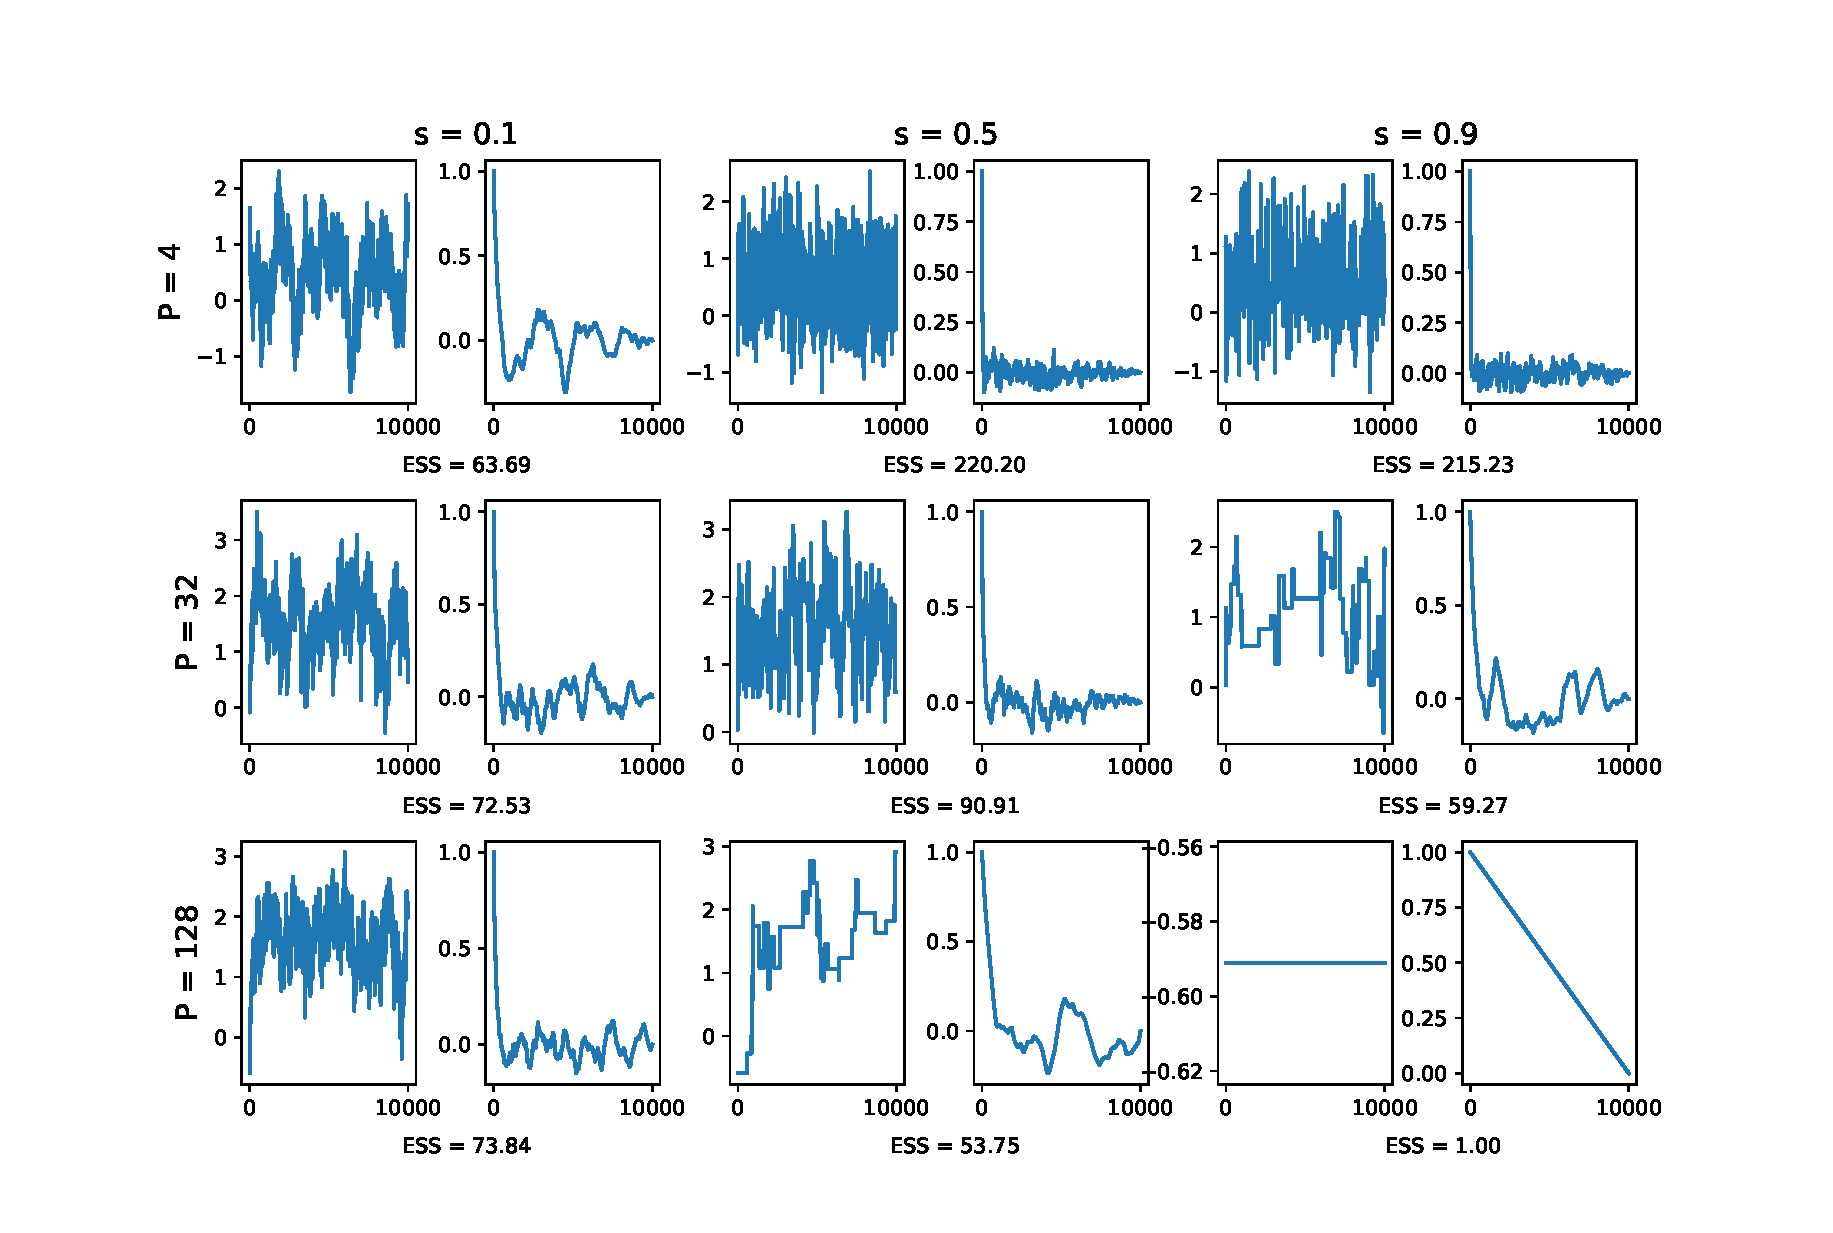
\includegraphics[width=\textwidth]{plots/RWM.eps}
    \caption{Trace plot (left), ACF (right) and ESS of the RWM algorithm for different values of \(P\) and \(s\).}
    \label{fig:RWM}
\end{figure}
The parameter \(s\), as well, is crucial for the performance of the RWM algorithm. If \(s\) is too small, the steps are too 
short, resulting in high autocorrelation and poor exploration of the parameter space. Conversely, if \(s\) is too 
large, the acceptance rate drops significantly, and the chain can get stuck. In both cases, the chain fails to mix 
adequately.\\
For low-dimensional problems, values like \(s = 0.5\) and \(s = 0.9\) work well, while $s=0.1$ hinder 
mixing. In higher dimensions, the choice of \(s\) is more critical, as larger values lead to a substantial drop 
in acceptance rates, causing the chain to stagnate in certain regions.\\
Despite these limitations, the RWM algorithm remains computationally efficient and easy to implement, making 
it a good choice for low-dimensional problems.
\\\\
\section{Preconditioned Crank-Nicholson}

Changing the proposal distribution to a Gaussian not centered in the current state, the pCN algorithm is a general Metropolis-Hastings algorithm that 
uses a preconditioner to improve the mixing of the chains. The proposal distribution is defined as follows:
\begin{equation}
    Q(\xi,\cdot) = \mathcal{N}(\sqrt{1-s^2}\xi , s^2 C) 
    \label{eq:pCN_proposal}
\end{equation}
where \(C\) is the same as in the RWM algorithm. The acceptance probability now depends also on the ratio of the proposal distributions, since 
the proposal is not centered in the current state and hence not symmetric.\\ \\
We now evaluate the performance of the pCN algorithm for different values of \(P\) and \(s\), comparing it with the RWM algorithm. \\
As shown in Figure \ref{fig:RWM}, the pCN algorithm exhibits behavior similar to the RWM algorithm, with performance depending on 
both dimensionality and the \(s\) parameter. While performance declines with increasing dimensionality, the pCN algorithm demonstrates 
greater robustness than the RWM algorithm in higher dimensions.
\begin{figure}[H]
    \centering
    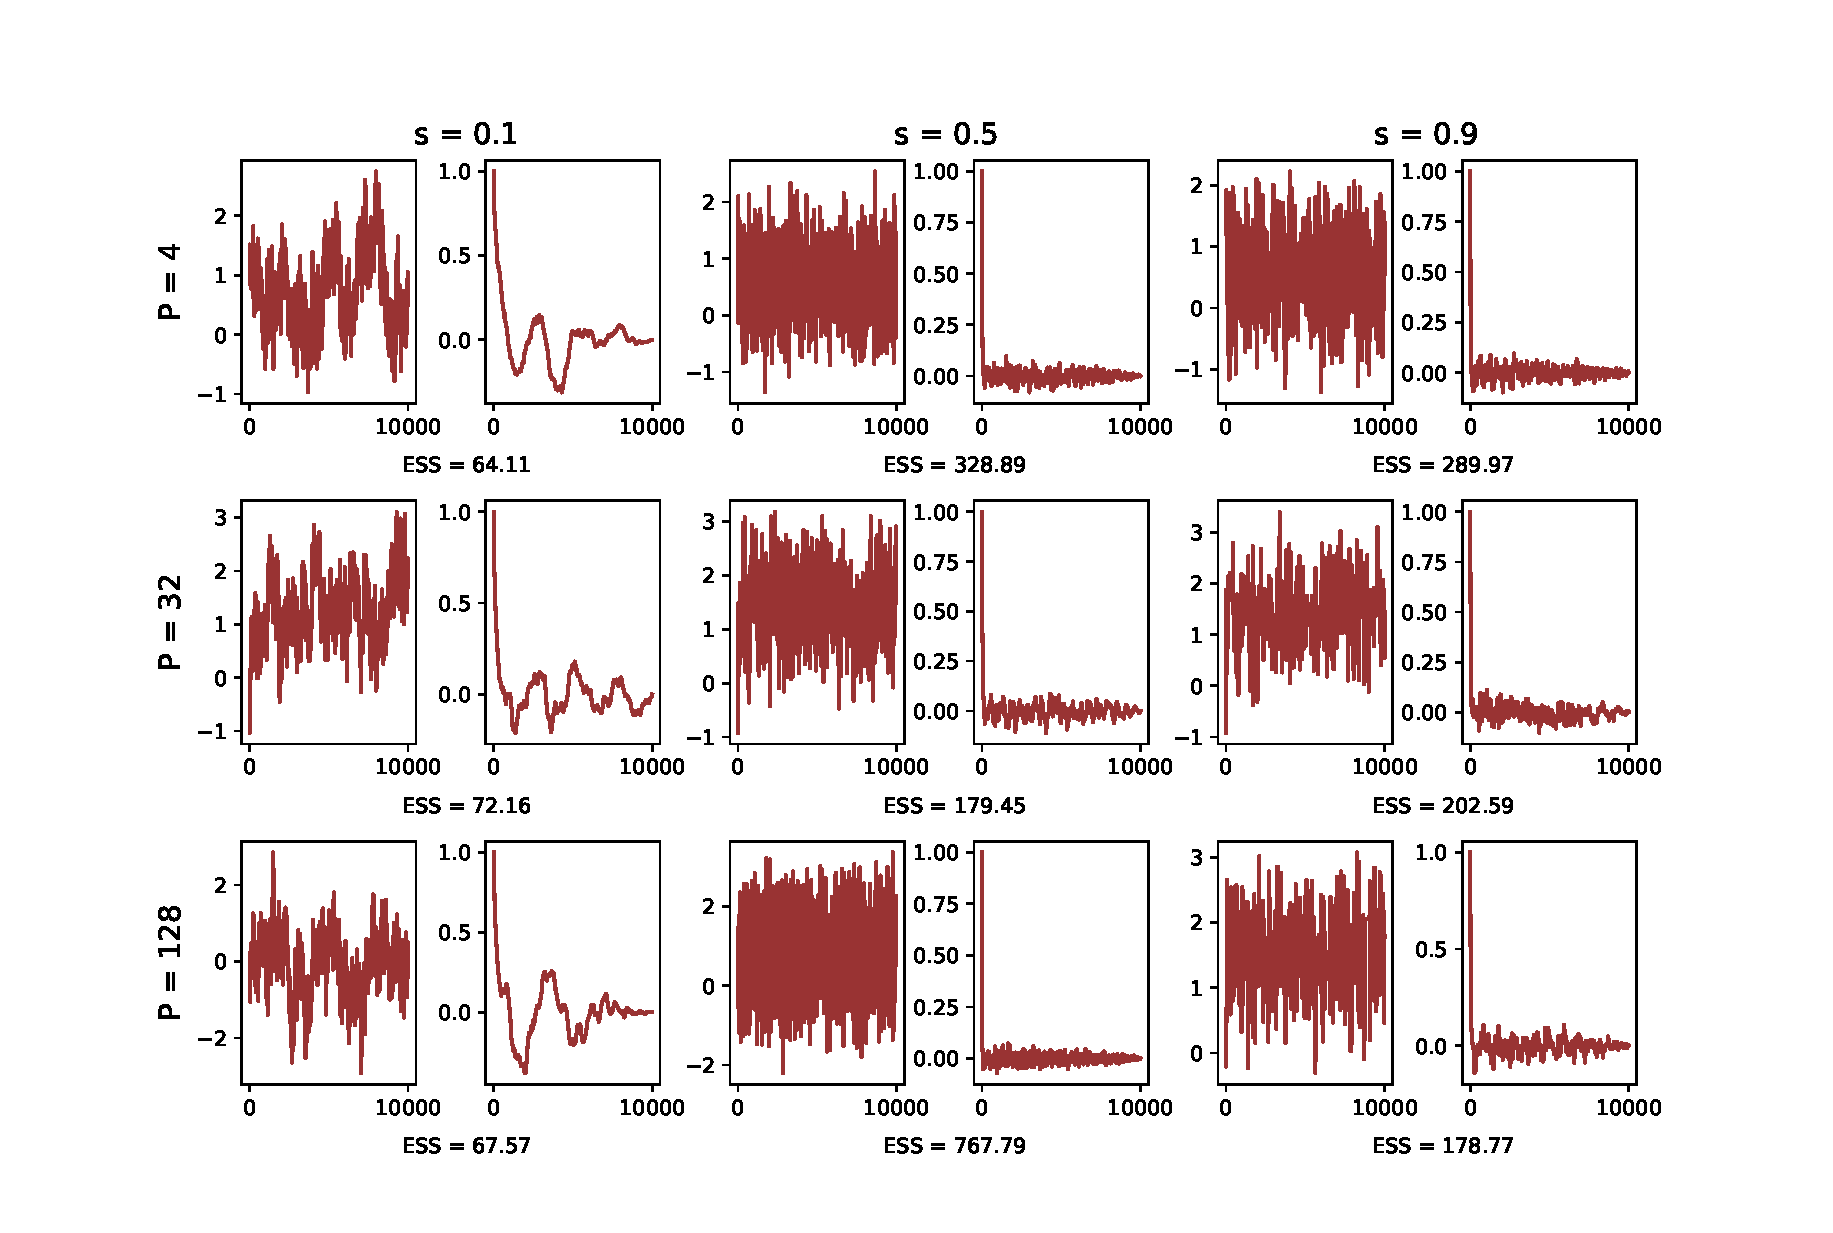
\includegraphics[width=\textwidth]{plots/pCN.eps}
    \caption{Trace plot (left), ACF (right) and ESS of the pCN algorithm for different values of \(P\) and \(s\).}
    \label{fig:pCN}
\end{figure}
Regarding the \(s\) parameter, the pCN algorithm is less sensitive than the RWM algorithm. Its acceptance 
rate remains more stable for moderate values of \(s\), and it is less prone to getting stuck. Extreme values 
of \(s\) can still lead to poor mixing or chain stagnation, but the effect is less severe compared to the RWM algorithm.\\
Although the pCN algorithm is computationally more demanding than the RWM algorithm, it offers improved robustness and 
efficiency in high-dimensional settings.

\section{Theoretical Analysis}

We now concentrate on some theoretical aspects of the problem.
\subsection*{(a)}
Firstly, we want to find an upper and lower bound for the likelihood function, when the integral function \(p(x)\) is discretized with,
for example, composite trapezoidal rule. Let's note with \(p_M(x)\) the function \(p(x)\), given by (\ref{eq:integral}), discretized on the grid 
$ \left\{ x_i = \frac{i}{M} \quad \text{with} \quad i = 0,1,\dots,M \right\}$. Let $n_x = \lfloor \frac{1}{x} \rfloor$, which denotes the index of the grid point closest to 
$x$ from below, we have that:
\begin{gather*}
    p_M(x) = \frac{e^{-u(0)}+2 \sum_{i=1}^{n_x-1}{e^{-u(x_{n_x})}} + e^{-u(1)} }{e^{-u(0)}+2 \sum_{i=1}^{M-1}{e^{-u(x_i)}} + e^{-u(1)}} \leq 1
\end{gather*}
since the exponential function is positive and $n_x \leq M$, hence the denominator is greater 
than the numerator. \\
We can now find the bounds for the discretized likelihood function \( \pi_M(y|\xi) \) of the expression (\ref{eq:likelihood})\\
The upper bound is immediate, exploiting the fact that 
an exponential with negative argument is always less than 1:
\begin{gather*}
    \pi_M(y|\xi) = \frac{1}{(\sqrt{2\pi}\sigma)^L}\exp\left(-\frac{1}{2\sigma^2}\sum_{i=1}^{L}{(y_i-p_M(x_i))^2}\right) \leq \frac{1}{(\sqrt{2\pi}\sigma)^L}
\end{gather*}
While for the lower bound, we can exploit the previous result:
\begin{gather*}
    \pi_M(y|\xi) = \frac{1}{(\sqrt{2\pi}\sigma)^L}\exp\left(-\frac{1}{2\sigma^2}\sum_{i=1}^{L}{(y_i-p_M(x_i))^2}\right) \geq \\
    \geq \frac{1}{(\sqrt{2\pi}\sigma)^L}\exp\left(-\frac{1}{2\sigma^2}\sum_{i=1}^{L}{\left(2y_i^2+2p_M(x_i)^2\right)}\right) \geq \\
    \geq \frac{1}{(\sqrt{2\pi}\sigma)^L}\exp\left(-\frac{1}{\sigma^2}\sum_{i=1}^{L}{\left(y_i^2 + 1\right)}\right) 
\end{gather*}
In conclusion, we have that the likelihood function is bounded by:
\begin{equation}
    \frac{1}{(\sqrt{2\pi}\sigma)^L}\exp\left(-\frac{1}{\sigma^2}\sum_{i=1}^{L}{\left(y_i^2 + 1\right)}\right) \leq \pi_M(y|\xi) \leq \frac{1}{(\sqrt{2\pi}\sigma)^L}
    \label{eq:likelihood_bounds}
\end{equation}

\subsection*{(b)}
Remark on notation, we will refer as $Q(\xi, \cdot)$ the Markov transition kernel of the pCN algorithm, expressed in (\ref{eq:pCN_proposal}), and with $q(\xi, \cdot)$ its probability density function.\\
\begin{itemize}
    \item {
    We can now prove that $Q$ and $\pi_0$ are in detailed balance, which requires (\ref{eq:det_bal}) to hold.
    \begin{equation}
        \int_{A}  Q(\xi,B) \pi_0(\xi) d\xi = \int_{B}  Q(\xi, A) \pi_0(\xi) d\xi \quad \forall A,B \in \mathcal{B}(\mathbb{R}^P)
        \label{eq:det_bal}
    \end{equation}
    We will instead prove the identity (\ref{eq:det_bal_pdf}), based on the pdf. 
    \begin{equation}
        \pi_0(\xi) q(\xi,\eta) = \pi_0(\eta) q(\eta, \xi)
        \label{eq:det_bal_pdf}
    \end{equation}
    In fact, it's trivial to see that (\ref{eq:det_bal_pdf}) implies (\ref{eq:det_bal}):
    \begin{gather*}
        \int_{A}  Q(\xi,B) \pi_0(\xi) d\xi = \int_{A}  \int_{B} q(\xi,\eta) \pi_0(\xi) d\eta d\xi = \int_{B} \int_{A}  q(\eta,\xi) \pi_0(\eta) d\xi d\eta = \int_{B}  Q(\eta,A) \pi_0(\eta) d\eta
    \end{gather*}
    Therefore, we can concentrate only on proving (\ref{eq:det_bal_pdf}). Recalling (\ref{eq:prior}), we have that:
    \begin{gather*}
    \frac{1}{\prod_{k=1}^P \sqrt{2 \pi k^{-2}}} \text{exp}\left( - \sum_{k=1}^P \frac{\xi_k^2 k^2} {2} \right) \frac{1}{\prod_{k=1}^P \sqrt{2 \pi k^{-2}}}  \text{exp} \left( - \sum_{k=1}^P \frac{( \eta_k - \sqrt{1-s^2}\xi_k)^2 k^2 } {2s^2} \right) = \\ = \frac{1}{\prod_{k=1}^P \sqrt{2 \pi k^{-2}}} \text{exp}\left( - \sum_{k=1}^P \frac{\eta_k^{2} k^2} {2} \right) \frac{1}{\prod_{k=1}^P \sqrt{2 \pi k^{-2}}}  \text{exp} \left( - \sum_{k=1}^P \frac{( \xi_k - \sqrt{1-s^2}\eta_k)^2 k^2 } {2s^2} \right)
    \end{gather*}
    The fraction terms simplify and we are left with
    $$
    \text{exp} \left( \sum_{k=1}^P - \frac{\xi_k^2 k^2} {2} - \frac{ \eta^{2}_k k^2 } {2s^2} + \frac{\sqrt{1-s^2}\xi_k\eta_k k^2}{s^2} - \frac{ \xi^2_k k^2 } {2s^2} + \frac{ \xi^2_k k^2 } {2}\right) =  
    $$
    $$
    = \text{exp} \left( \sum_{k=1}^P - \frac{\eta_k^{2} k^2} {2} - \frac{ \xi^{2}_k k^2 } {2s^2} + \frac{\sqrt{1-s^2}\eta_k\xi_k k^2}{s^2} - \frac{ \eta^{2}_k k^2 } {2s^2} + \frac{ \eta^{2}_k k^2 } {2}\right)
    $$
    Canceling out the equal terms we obtain the following identity
    $$
    \text{exp} \left( \sum_{k=1}^P - \frac{ \eta^{2}_k k^2 } {2s^2} + \frac{\sqrt{1-s^2}\xi_k\eta_k k^2}{s^2} - \frac{ \xi^2_k k^2 } {2s^2} \right) =  \text{exp} \left( \sum_{k=1}^P - \frac{ \eta^{2}_k k^2 } {2s^2} + \frac{\sqrt{1-s^2}\xi_k\eta_k k^2}{s^2} - \frac{ \xi^2_k k^2 } {2s^2} \right) 
    $$
    thus verifying the detailed balance condition.}\\
\item{
    We want now to determine the acceptance rate for the pCN algorithm. To do so, we would typically 
    need the posterior distribution, which is given by (\ref{eq:posterior}). However, in our implementation, we do not have access to the true likelihood; 
    instead, we only have access to its discretized version. Therefore, the posterior distribution is 
    approximated using the discretized likelihood and the prior, as follows:
    \begin{gather*}
        \pi_M(\xi) = \frac{\pi_M(y|\xi)\pi_0(\xi)}{\pi(y)} 
    \end{gather*}
    In this setting, the acceptance rate for the pCN algorithm is given by:
    \begin{gather*}
        \alpha(\xi,\eta) = \min\left\{1, \frac{\pi_M(\eta)q(\eta,\xi)}{\pi_M(\xi)q(\xi,\eta)} \right\} =
        \min\left\{1, \frac{\pi_M(y|\eta)\pi_0(\eta)q(\eta,\xi)}{\pi_M(y|\xi)\pi_0(\xi)q(\xi,\eta)} \right\}=\\
        = \min\left\{1, \frac{\pi_M(y|\eta)}{\pi_M(y|\xi)} \right\}
    \end{gather*}
    where we exploited (\ref{eq:det_bal_pdf}).}\\
\item{
    With this form, we can compute a lower bound for the acceptance rate. Given (\ref{eq:likelihood_bounds}), we have that:
    \begin{gather*}
        \frac{\pi_M(y|\eta)}{\pi_M(y|\xi)} \geq \exp\left(-\frac{1}{\sigma^2}\sum_{i=1}^{L}{\left(y_i^2 + 1\right)}\right)
    \end{gather*}
    we have that the acceptance rate is bounded from below by the exponential function above. In fact:
    \begin{gather*}
        \alpha(\xi,\eta) = \min\left\{1, \frac{\pi_M(y|\eta)}{\pi_M(y|\xi)} \right\} \geq \min\left\{1, \exp\left(-\frac{1}{\sigma^2}\sum_{i=1}^{L}{\left(y_i^2 + 1\right)}\right) \right\}=
        \exp\left(-\frac{1}{\sigma^2}\sum_{i=1}^{L}{\left(y_i^2 + 1\right)}\right)
    \end{gather*}}
\end{itemize}

\section{Laplace's Approximation}
We now introduce Laplace's approximation to improve the performance of the MCMC algorithms. Laplace approximation is a common technique in Bayesian statistics 
used to approximate complex posterior distributions. It relies on the idea that, for a well-behaved posterior, a second-order Taylor expansion around the 
maximum a posteriori (MAP) estimate provides a good approximation. Specifically, if \(\pi(\xi)\) is the posterior distribution, the MAP estimate \(\xi_{\text{map}}\) 
is defined as:
\begin{equation*}
    \xi_{\text{map}} = \arg \min_{\xi} (-\log \pi(\xi))
\end{equation*} 
Using a second-order Taylor expansion, the posterior \(\pi(\xi)\) around \(\xi_{\text{map}}\) is approximated by a Gaussian 
distribution with mean \(\xi_{\text{map}}\) and covariance given by the inverse of the Hessian matrix \(H\) of the negative log-posterior 
evaluated at \(\xi_{\text{map}}\).\\\\
In MCMC, Laplace’s approximation can be used to construct a proposal distribution for the Metropolis-Hastings algorithm. 
In this case, we implement an independence sampler, which is a special case of the Metropolis-Hastings algorithm where the proposal distribution is independent from the current state:
\begin{equation*}
    Q(\xi,\cdot) = Q(\cdot) = \mathcal{N}(\xi_{\text{map}}, H^{-1})
\end{equation*}
Where $H^{-1}$ is the inverse of the Hessian matrix of the negative log-posterior evaluated in $\xi_{map}$\\
Computationally, this is implemented with BFGS optimization algorithm, which is a quasi-Newton method used to minimize differentiable functions. Unlike the Newton method, which requires explicit 
computation of the Hessian matrix, BFGS approximates it iteratively using gradient information, making it computationally more efficient.
It gives us the MAP estimate and a low rank approximation of the Hessian matrix, which we use to construct the proposal distribution.\\\\
We repeated the analysis previously conducted for the RWM and pCN algorithms using Laplace's approximation. 
As shown in Figure \ref{fig:Laplace}, contrary to our expectations, Laplace's approximation does not improve 
the performance of the MCMC algorithms. Although it performs well in low dimensions, for higher ones the ESS values are not as low as those for RWM, 
and the plot reveals that the chain encounters issues and gets stuck. Additionally, in terms of runtime, Laplace's approximation is 
less efficient than the other algorithms. It does not appear to be a suitable choice for this problem, though it 
is important to note that we are performing inference with a very small number of observations, and this method 
may lack accuracy in such a setting.

\begin{figure}[H]
    \centering
    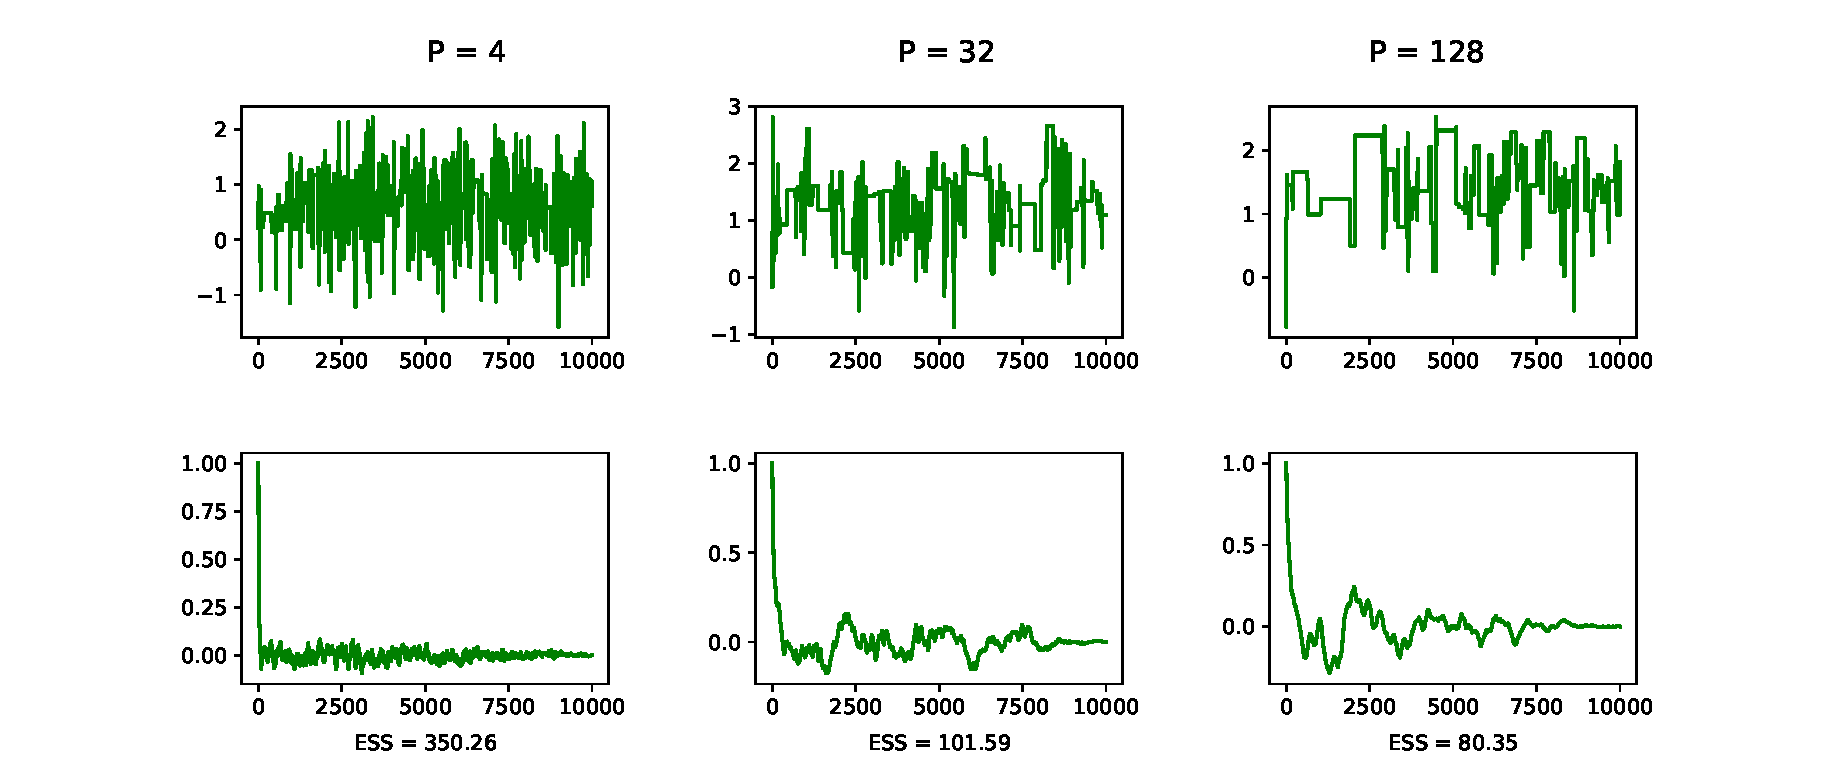
\includegraphics[width=\textwidth]{plots/Laplace.eps}
    \caption{Trace plot (top), ACF (bottom) and ESS of the Laplace's approximation algorithm with increasing dimensionality \(P\).}
    \label{fig:Laplace}
\end{figure}

\section{Estimation of a Quantity of Interest}
We are now interested in exploiting MCMC methods to estimate a function $q(\xi)$, specifically the integral of the permeability:
\begin{equation*}
    q(\xi) = \int_0^1{e^{-u(x,\xi)} dx}
\end{equation*}
We discretized the integral with trapezoidal rule and used the pCN algorithm with \(s = 0.5\), as this value yielded the best results 
in the previous analysis. The algorithm was run for various values of \(P\), and for
each chain, the estimator was calculated as the mean of the chain, excluding the 
initial transient phase with a burn-in of \(B = 50\). The behavior of the chains are presented in 
Figure \ref{fig:Integral}. As we can see, the three chains are well-mixed, even in large
dimensions. 
\begin{figure}[H]
    \centering
    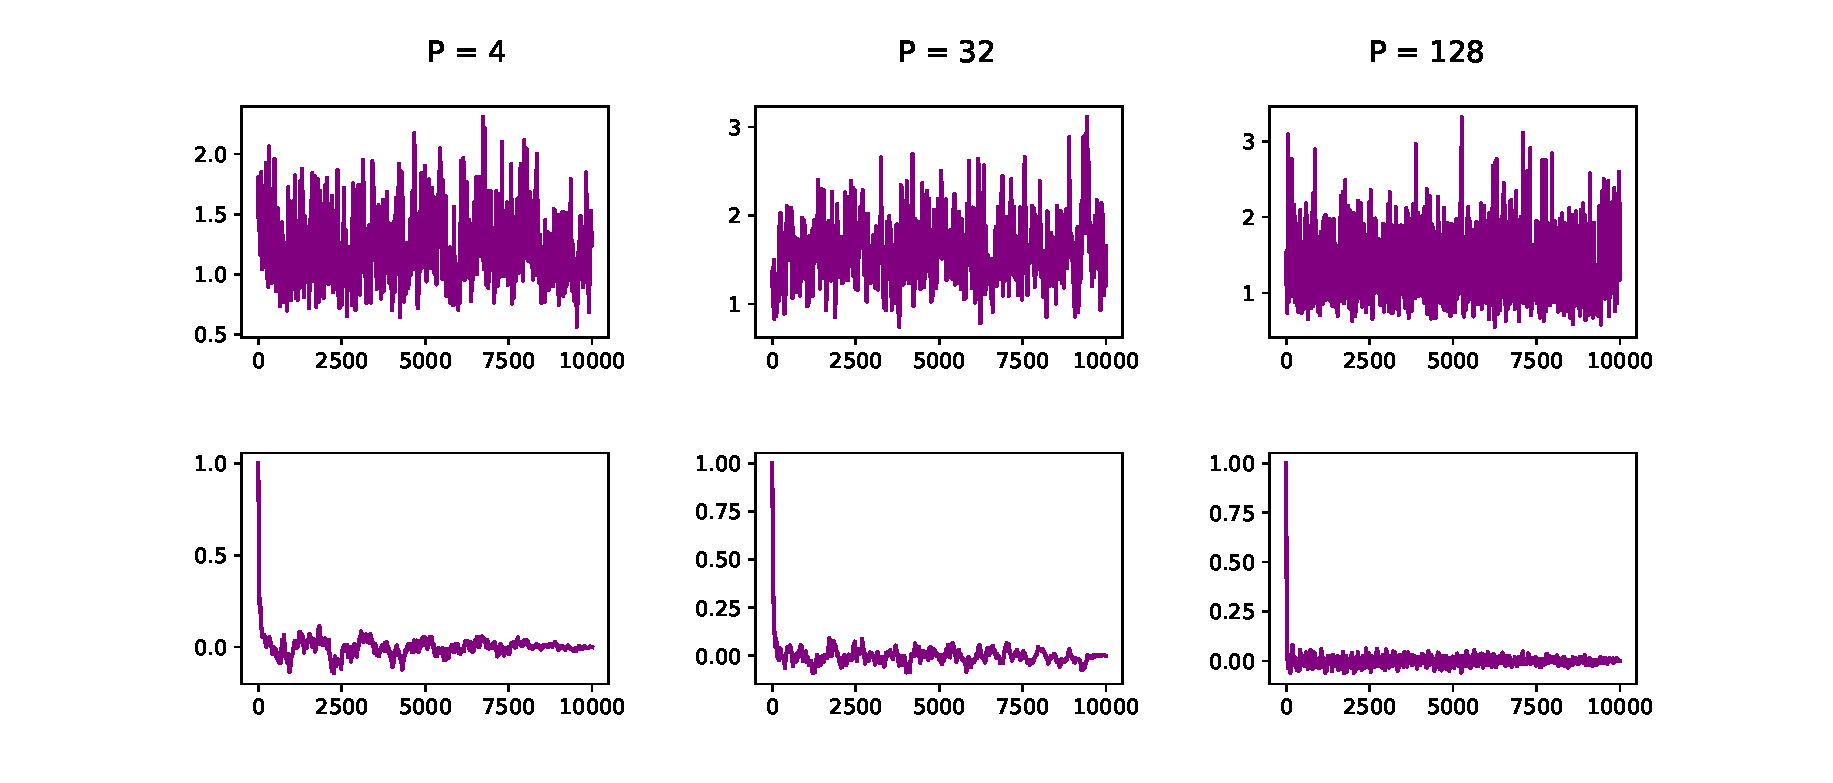
\includegraphics[width=\textwidth]{plots/Integral.eps}
    \caption{Trace plot (top) and ACF (bottom) of the pCN algorithm with increasing dimensionality \(P\) 
    for estimation of the quantity $q(\xi)$.}
    \label{fig:Integral}
\end{figure}
Nonetheless, the estimation of the quantity \(q(\xi)\) is challenging, as the
estimations are not robust and show high variability with the chose of $P$, as Table \ref{tab:q_estimation} shows. This, again,
could be due to the small number of observations, which makes the problem ill-posed. 
\begin{table}[h!]
    \centering
    \begin{tabular}{|c|c|c|c|}
    \hline
    $P$ & 4 & 32 & 128 \\ \hline
    $q(\xi)$ & 1.21011 & 1.57575  & 1.29133   \\ \hline
    \end{tabular}
    \caption{Values of $q(\xi)$ estimated with pCN.}
    \label{tab:q_estimation}
\end{table}
    
However, we are interested in the Mean Squared Error (MSE) of this estimator, when chosen the dimensionality. \\
We fixed $P=32$ and we ran $K=100$ simulations. For every simulation, we computed the estimator $\hat{q}(\xi)$, and in the end we calculated the estimantion of the MSE as follows:
\begin{equation*}
    \hat{\text{MSE}}(\hat{q}(\xi)) = \frac{1}{K-1} \sum_{i=1}^{K}{(\hat{q}(\xi_i) - \hat{\mu}_{q})^2} \quad \text{where} \quad \hat{\mu}_{q} = \frac{1}{K} \sum_{i=1}^{N}{\hat{q}(\xi_i)}
\end{equation*}
The value we obtained is $\hat{\text{MSE}}= 0.000811$, that
is notably small, indicating a high degree of consistency in the estimator.

\section{Analysis with more observations}

Up to now, we have considered the case where the number of observations was very limited, specifically 4. We now analyze how the performance of the algorithms
changes when the number of observations increases. We consider 39 observations, randomly generated as follows:
\begin{gather*}
    y_i = p(i/40,\xi) + \eta_i \quad \text{where} \quad \eta_i \overset{\text{iid}}{\sim} \mathcal{N}(0,\sigma^2) \quad \forall i=1,\dots,39
\end{gather*}
considering a possible realization of $\xi$ from the prior. \\
We repeated the previous analysis in the same order. We will not comment on the runtimes, as they all increased compared 
to the earlier case, but their relative behavior remains consistent.\\

\begin{itemize}

\item{
    In this case, the RWM algorithm performs unexpectedly worse than with 4 observations, as shown in Figure \ref{fig:RWM2}. For every
    value of \(P\) and \(s\), the algorithm struggles to explore the parameter space effectively.
    The ESS values are exceptionally low, approaching zero in most instances, and the chains exhibit poor mixing, which is 
    particularly evident in the ACF plots. This behavior is likely due to the increased complexity of the problem with more
    observations. 
    \begin{figure}[H]
        \centering
        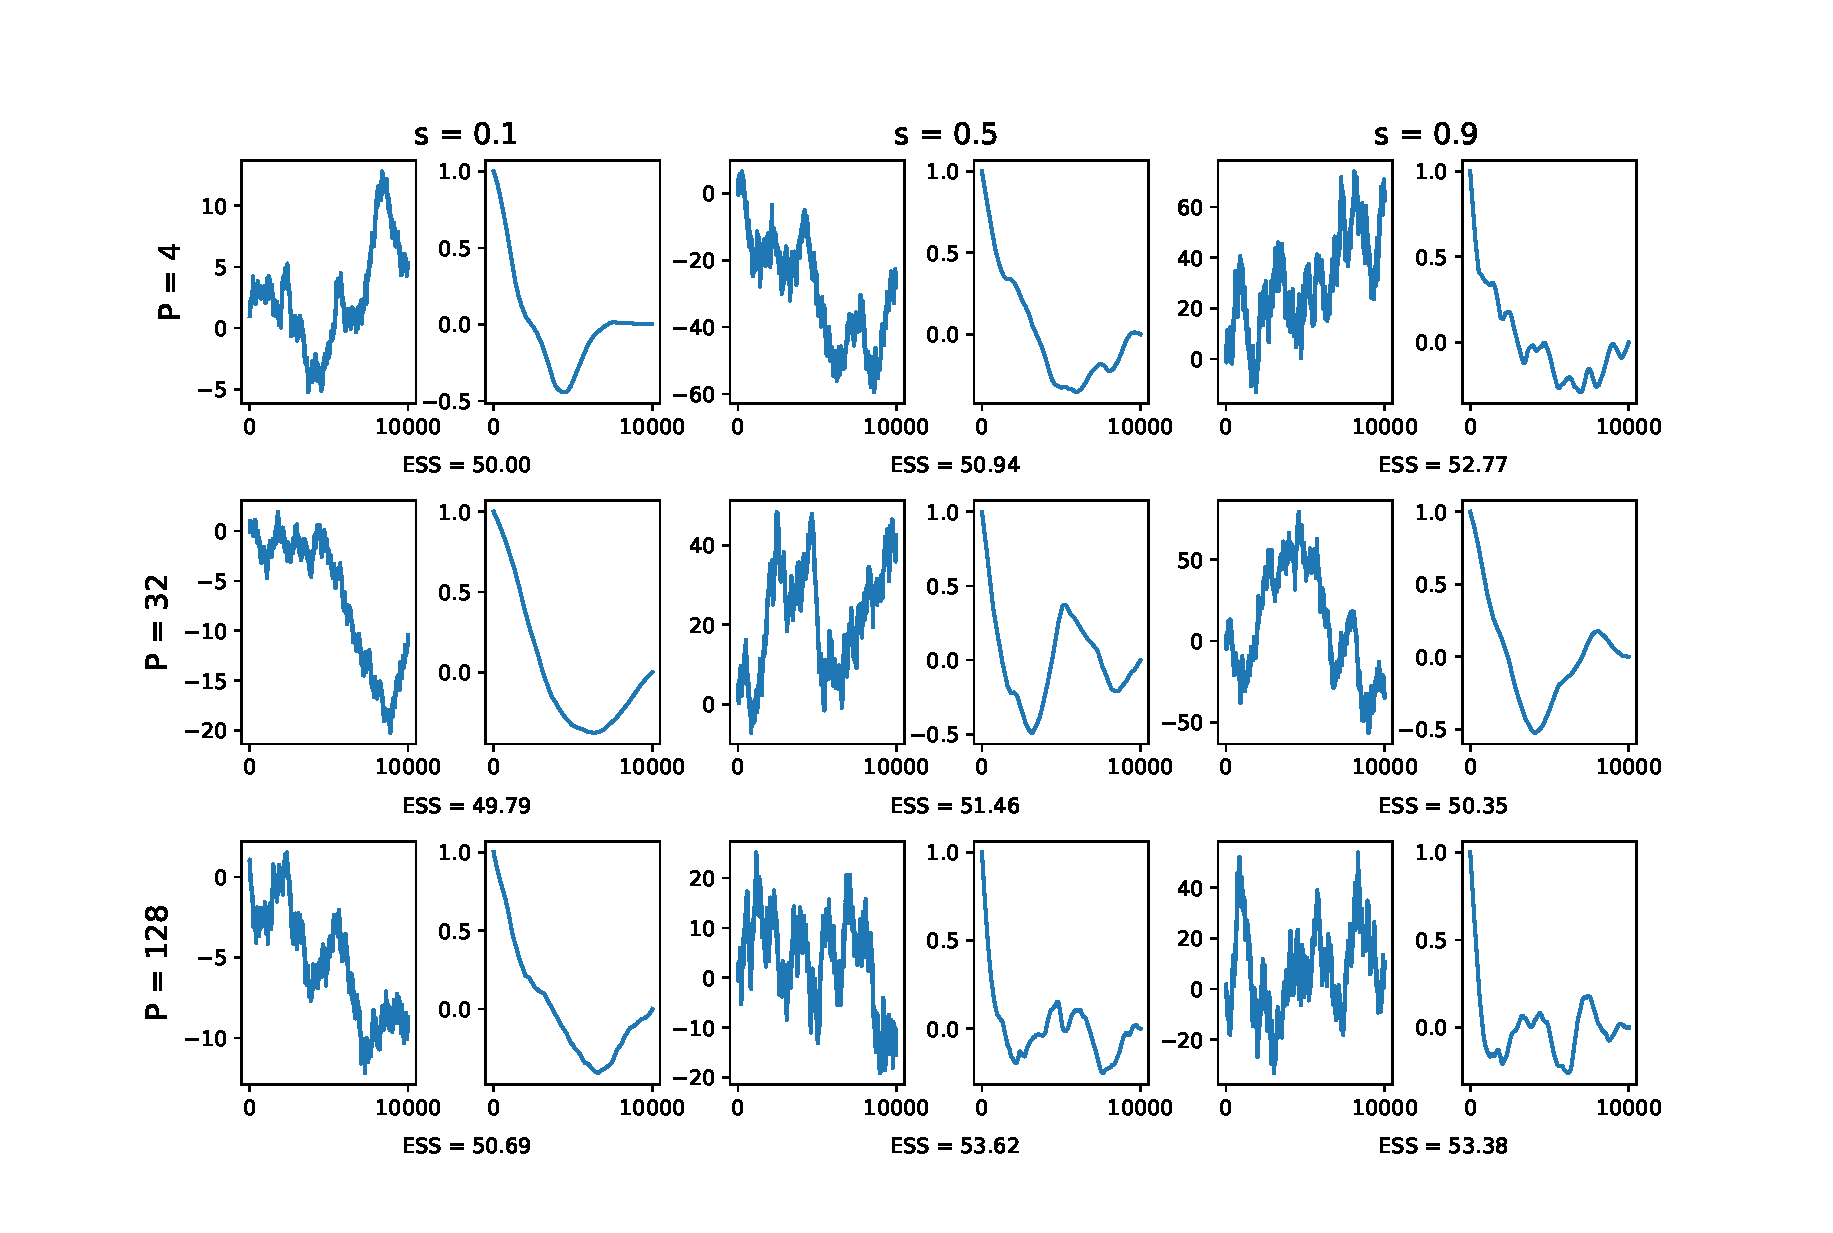
\includegraphics[width=\textwidth]{plots/RWM2.eps}
        \caption{Trace plot (left), ACF (right) and ESS of the RWM algorithm with 39 observations for different values of \(P\) and \(s\).}
        \label{fig:RWM2}
    \end{figure}
}

\item{
    The pCN algorithm, by contrast, demonstrates improved performance with 39 observations, as shown 
    in Figure \ref{fig:pCN2}. In this scenario, the dimensionality \(P\) has a reduced impact on the 
    algorithm's efficiency, and the chains display better mixing behavior. However, the ESS slightly 
    decreases as \(P\) increases. The choice of \(s\) remains critical, with the higher value \(s=0.9\) 
    now being preferable. Conversely, with \(s=0.1\), the algorithm struggles to effectively explore 
    the parameter space.
    \begin{figure}[H]
        \centering
        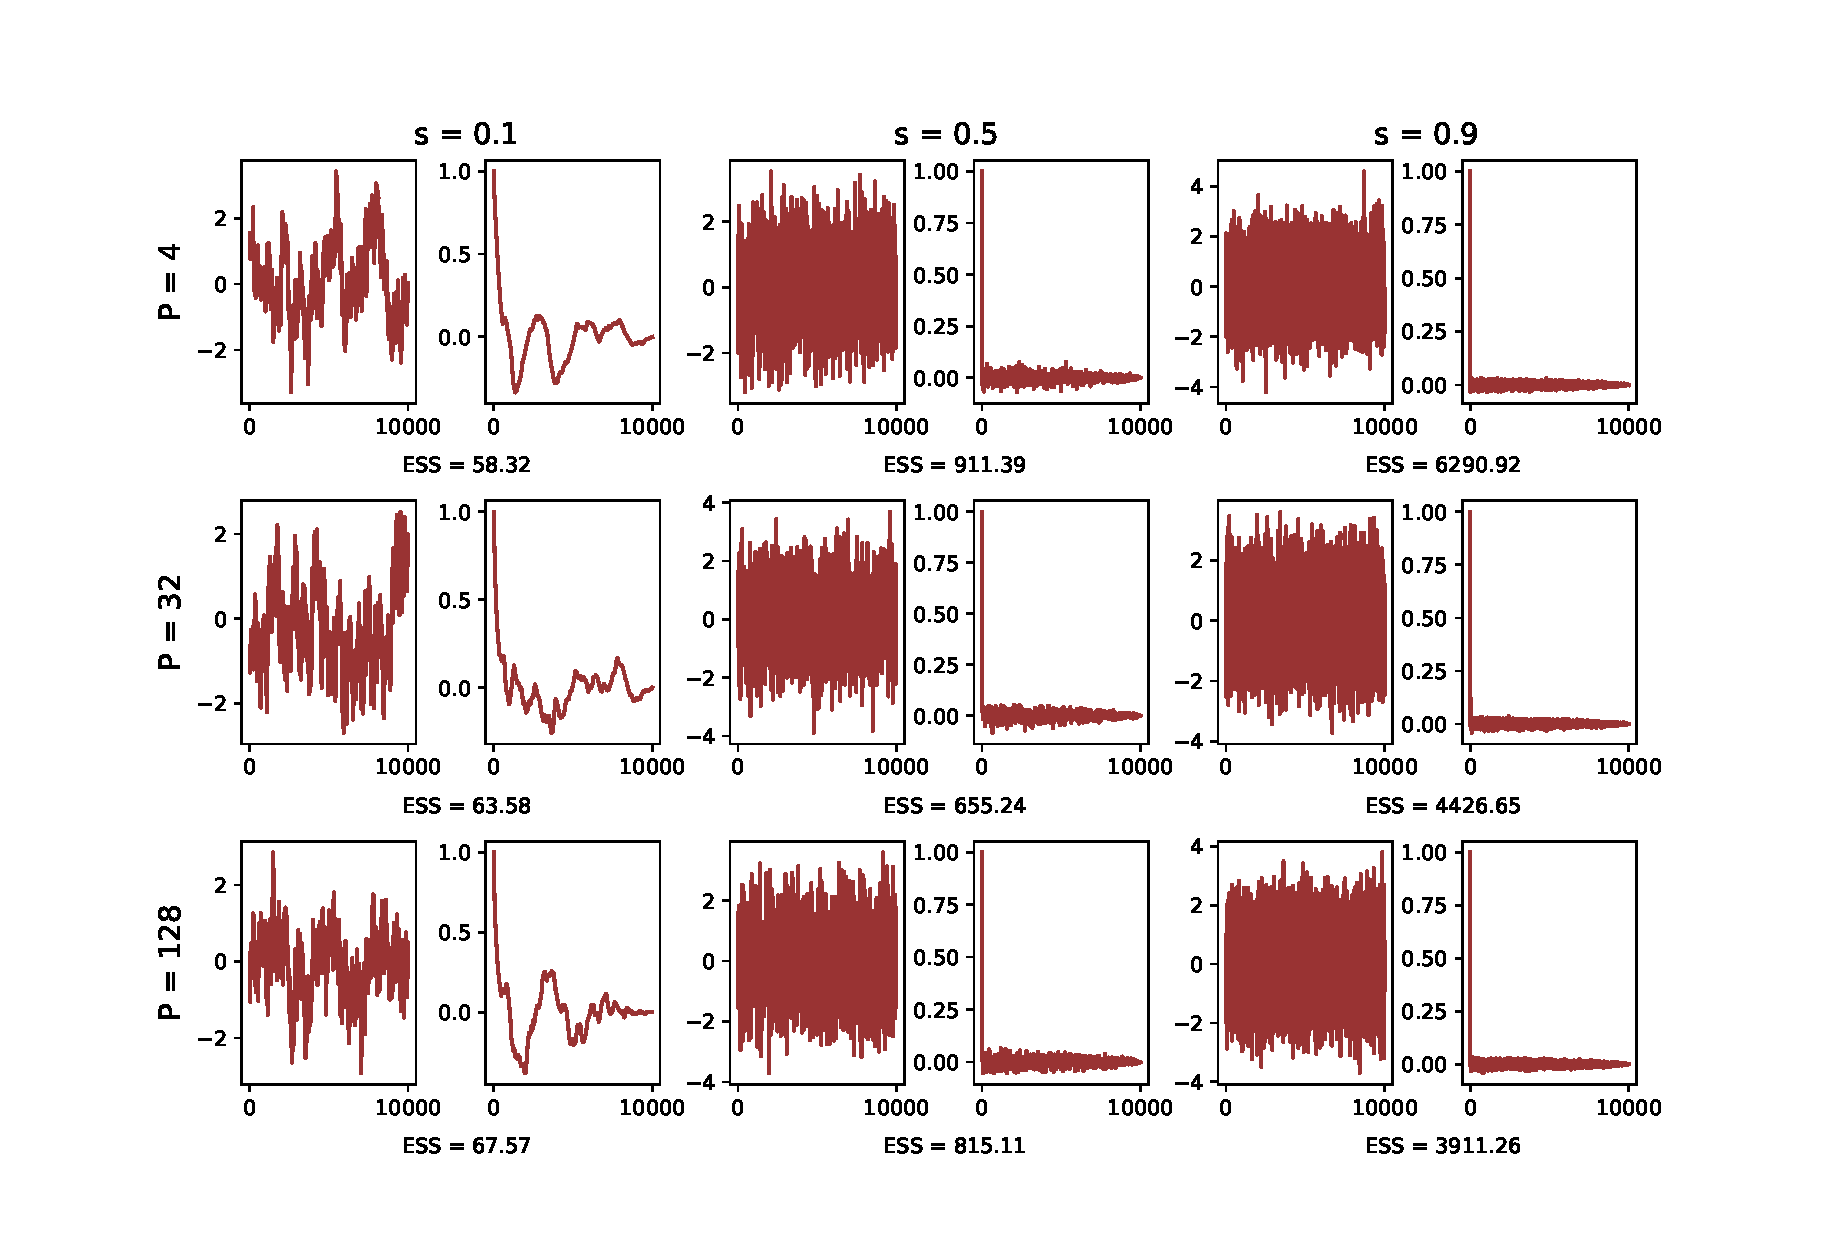
\includegraphics[width=0.8\textwidth]{plots/pCN2.eps}
        \caption{Trace plot (left), ACF (right) and ESS of the pCN algorithm with 39 observations for different values of \(P\) and \(s\).}
        \label{fig:pCN2}
    \end{figure}
}

\item{
    As we expected, Laplace's approximation really improves the performance of the MCMC algorithms with 39 observations, as shown in Figure \ref{fig:Laplace2}.
    The ESS values are incredibly high ($\approx N$) and the chains mix well, even in high dimensions. This is a significant improvement over the previous cases, 
    where Laplace's approximation did not perform well. 
    \begin{figure}[H]
        \centering
        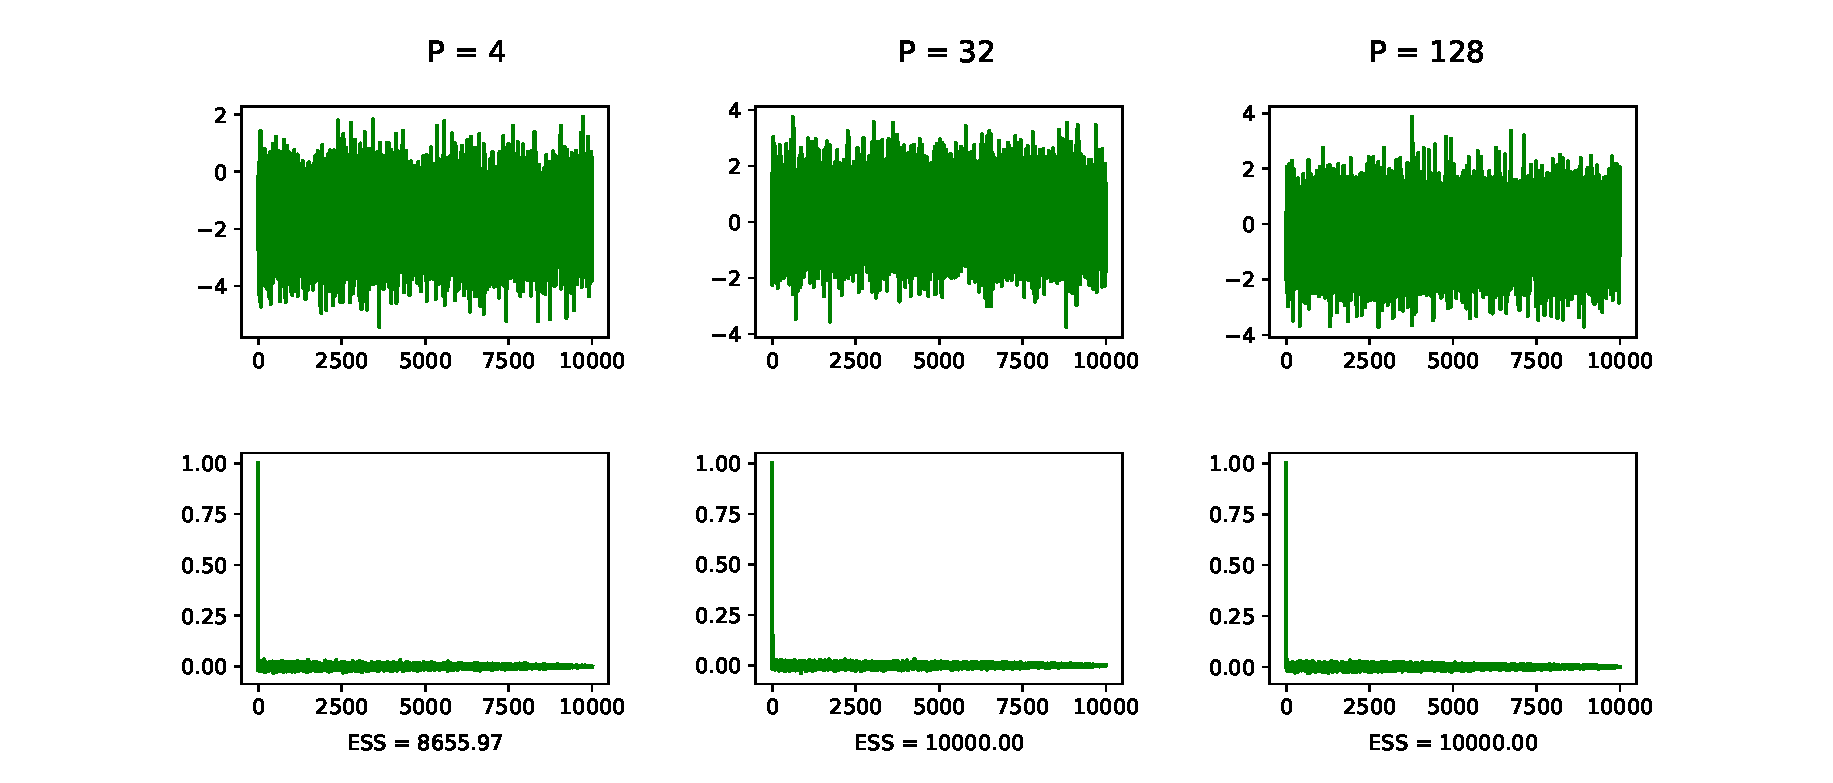
\includegraphics[width=0.9\textwidth]{plots/Laplace2.eps}
        \caption{Trace plot (top), ACF (bottom) and ESS of the Laplace's approximation algorithm with 39 observations with increasing dimensionality \(P\).}
        \label{fig:Laplace2}
    \end{figure}
}

\item{
    Finally, we repeated the estimation of the quantity \(q(\xi)\) with the pCN algorithm for 39 observations. We implemented again 
    pCN with $P=32$ but now considering $s=0.9$ because it showed to best impact on the performance. The behavior of the chains are shown in Figure \ref{fig:Integral2}, and
    we see that the chains are well-mixed, even in high dimensions. 

    \begin{figure}[H]
        \centering
        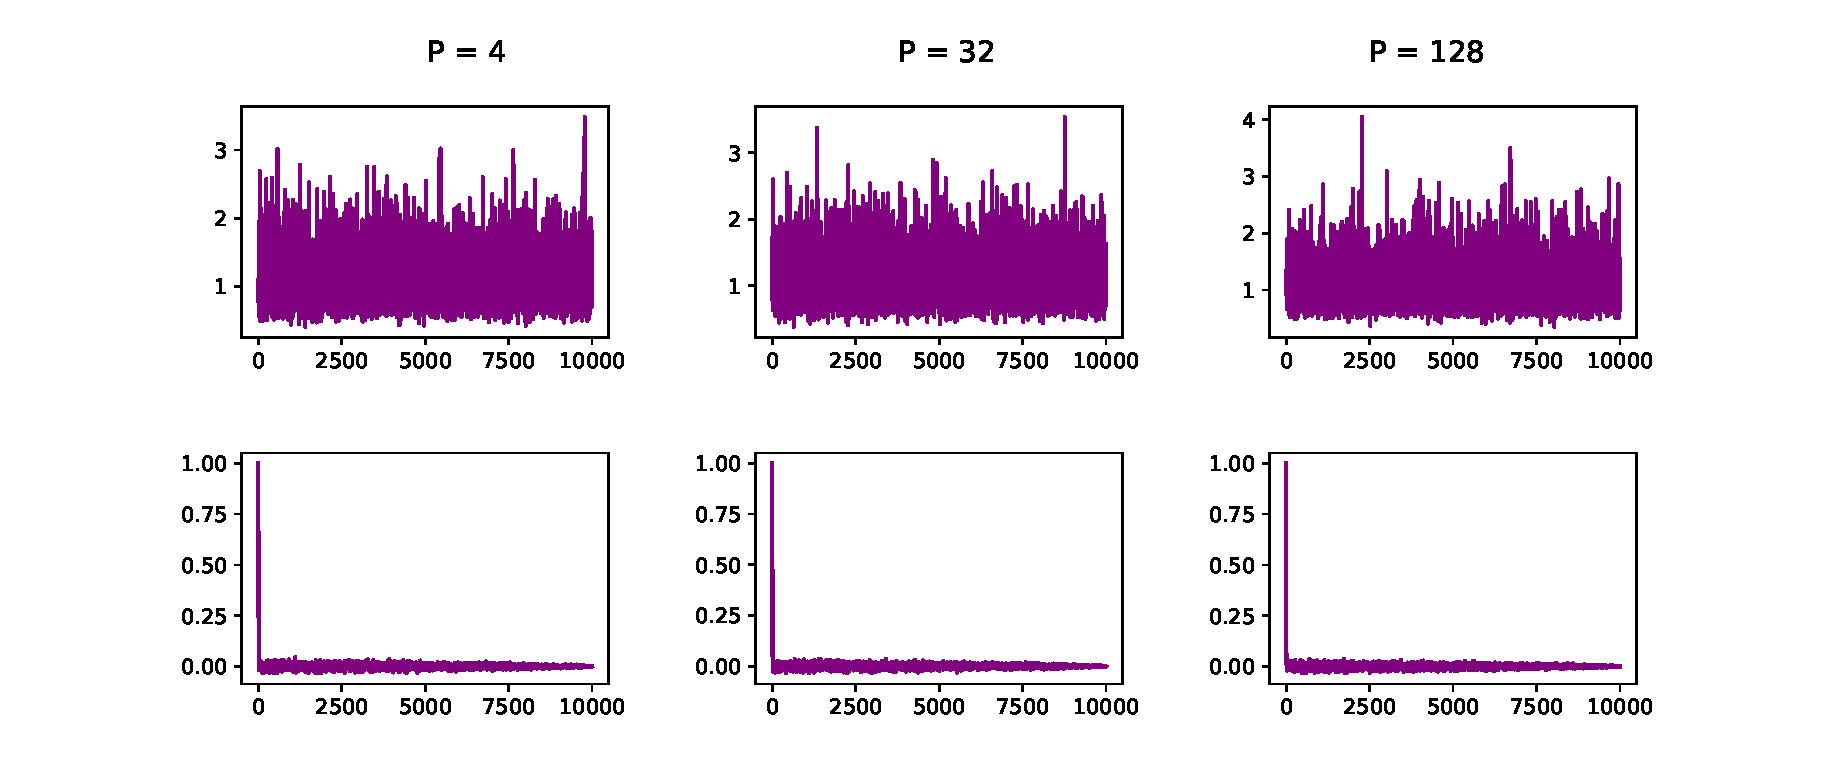
\includegraphics[width=\textwidth]{plots/Integral2.eps}
        \caption{Trace plot (top) and ACF (bottom) of the pCN algorithm with 39 observations with increasing dimensionality \(P\) 
        for estimation of the quantity $q(\xi)$.}
        \label{fig:Integral2}
    \end{figure}
    
    Moreover, the estimation of the quantity \(q(\xi)\) is more robust than in the previous cases, as shown in Table \ref{tab:q_estimation2}.
    The values are more consistent across different values of \(P\), and the variability is reduced. 

    \begin{table}[H]
        \centering
        \begin{tabular}{|c|c|c|c|}
        \hline
        $P$ & 4 & 32 & 128 \\ \hline
        $q(\xi)$ & 1.07433 & 1.08428  & 1.08977   \\ \hline
        \end{tabular}
        \caption{Values of $q(\xi)$ estimated with pCN with 39 observations.}
        \label{tab:q_estimation2}
    \end{table}

    Finally, we calculated the MSE of the estimator, as we did before. The value we obtained is $\hat{\text{MSE}}= 0.00109$, that 
    is higher than before, but still small, indicating a high degree of consistency in the estimator.
}

\end{itemize}

\section*{Conclusions}

Our analysis of Bayesian inverse problems in high-dimensional spaces provides valuable insights into the performance and scalability of MCMC algorithms, 
focusing on the optimal choice of the proposal distribution depending on the problem's complexity: dimensionality and number of observations.\\
The Random Walk Metropolis (RWM) proves useful in simple settings due to its computational efficiency. However, to achieve good performance, 
it is crucial to work with a limited number of observations, carefully choose the parameter \( s \), and work in low-dimensional spaces. 
In more complex cases, the method shows significant limitations, such as low Effective Sample Size (ESS) values and poor chain mixing.\\
The Preconditioned Crank-Nicholson (pCN) method stands out as the most robust among the methods analyzed. It performs well with both few and many observations, 
maintaining good mixing ability even in high-dimensional spaces. However, the parameter \( s \) must be chosen carefully to balance the trade-off 
between acceptance and exploration of the spatial parameter, especially when the number of observations is limited.\\
Laplace's approximation, based on Bayesian statistical approximation, is highly dependent on the number of observations. With a limited number of data points, 
it fails to reach its full potential and performs worse than the other algorithms. However, with a sufficient number of observations, 
it shows excellent mixing capabilities and very high ESS values, even when $P \rightarrow \infty$, making it an optimal choice in such contexts.\\
To conclude, we can assert that the choice of the MCMC algorithm is crucial to the performance of the overall method. 
Each algorithm should be selected after a thorough analysis of the problem's specific characteristics, as this ensures 
the method is tailored to the dataset and objectives at hand.
\end{document}
